\section{Аналитический раздел} \label{analysis}

Аналитический раздел курсовой работы является важным этапом проектирования приложения, поскольку он определяет основные требования к системе и выбирает наиболее подходящую модель базы данных. В данном разделе будут рассмотрены различные типы баз данных, их преимущества и недостатки, а также проведен анализ существующих систем управления базами данных. На основе полученных результатов будет выбрана оптимальная модель базы данных для реализации приложения. Кроме того, в данном разделе будут определены пользователи системы, формализованы данные и представлены сущности, что позволит более точно определить требования к приложению и разработать его структуру.

\subsection{Требования к приложению}

Чтобы спортсмены имели возможность сразу же после выхода из воды взвесить улов, подсчет очков и судейство происходит прямо на берегу водоемов, зачастую в полевых условиях, где возможность оборудовать рабочее место с ноутбуком предоставляется редко. Разрабатываемое приложение было бы удобно использовать на более компактных устройствах, таких как телефон или планшет. В связи с чем выбор пал на платформу iOS \cite{ios} --- создаваемое программное обеспечение будет разработано для смартфонов и электронных планшетов компании Apple \cite{apple}.

Приложение должно поддерживать определенный функционал:
\begin{itemize}[label=---]
	\item возможность входа без авторизации для спортсменов;
	\item персонализация для судей и администраторов;
	\item формирование соревнований и их этапов;
	\item создание команд, деление участников по командам;
	\item добавление информации об улове участников;
	\item подсчет очков участников, команд;
	\item формирование личного и командного рейтингов;
	\item поиск определенного участника или конкретной команды.
\end{itemize}

\subsection{Пользователи системы}

В приложении будут представлены следующие роли:
\begin{enumerate}
	\item Участник --- пользователь, обладающий возможностью просматривать командный и личный рейтинги по любым этапам соревнований, устанавливать параметры поиска, а также искать профили конкретных участников и команд. Роль не требует авторизации.
	\item Судья — пользователь, обладающий возможностями участника, а также возможностью создавать и удалять соревнования, создавать, редактировать и удалять участников, команды, добавлять участников в команды и удалять из команд, добавлять, редактировать и удалять уловы участников в этапы соревнований. Роль требует авторизации.
	\item Администратор --- пользователь, обладающий возможностями участника и судьи, а также возможностью редактировать и удалять профили судей. Роль требует авторизации.
\end{enumerate}

На рисунке \ref{fig:UseCase} представлена диаграмма использования приложения.

\begin{figure}[h!]
	\centering{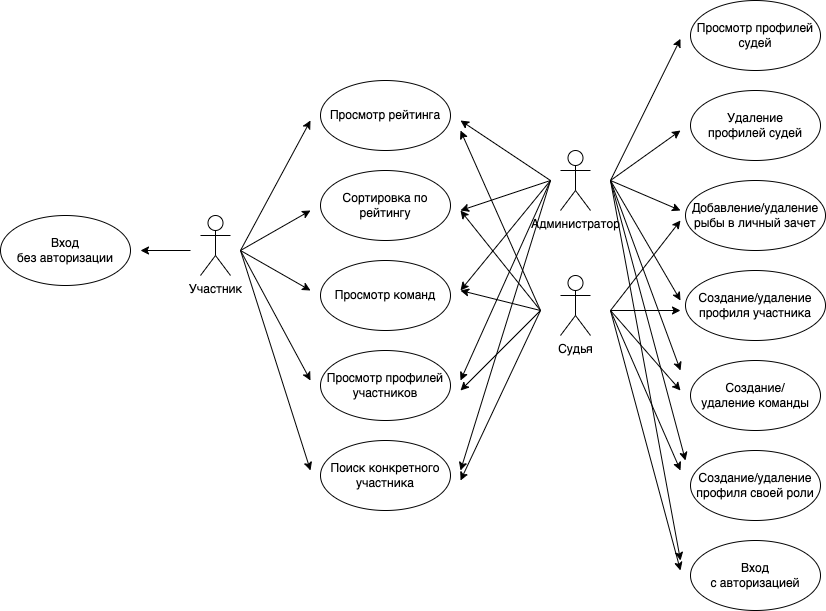
\includegraphics[scale=0.5]{img/UseCase.png}}
	\caption{Диаграмма использования приложения}
	\label{fig:UseCase}
\end{figure}

\subsection{Формализация данных}

База данных должна хранить информацию о следующих сущностях:

\begin{itemize}[label=---]
	\item соревнование;
	\item команда;
	\item участник;
	\item этап;
	\item улов;
	\item пользователь;
	\item авторизация.
\end{itemize}

В таблице \ref{decisions} представлены сущности и сведения о них.

\begin{table}[ht!]
	\centering
	\caption{Сущности и сведения о них}
	\label{decisions}
	\begin{tabular}{|p{4.3cm}|p{10.3cm}|}
		\hline
		\textbf{Сущность} & \textbf{Сведения}\\
		\hline 
		\ Участник & Фамилия, имя, отчество, команда, город, дата рождения, очки \\
		\hline 
		\ Команда & Название, соревнования, очки \\
		\hline 
		\ Соревнования & Название, команды \\
		\hline 
		\ Этап & Название этапа, участник, соревнование, очки \\
		\hline 
		\ Улов & Рыба, этап, вес, очки \\
		\hline 
		\ Пользователь & Роль, авторизация  \\
		\hline 
		\ Авторизация & Логин, пароль \\
		\hline
	\end{tabular}
\end{table}

\subsection{Анализ моделей баз данных}

Одним из ключевых этапов разработки приложения является выбор модели базы данных, которая будет использоваться для хранения и управления данными. Существует множество различных типов баз данных  совместимых с iOS, каждый из которых имеет свои преимущества и недостатки. Далее будут рассмотрены основные типы баз данных, проведен анализ существующих систем управления базами данных и выбрана наиболее подходящую модель для реализации приложения. Кроме того, будет определен пользователи системы, формализованы данные и представлены сущности, чтобы более точно определить требования к приложению и разработать его структуру.

\subsubsection{Реляционная модель}

Реляционная модель базы данных --- это способ организации данных, в котором информация хранится в виде таблиц, состоящих из строк и столбцов. Каждая таблица представляет отдельную сущность или объект, а каждая строка в таблице --- это конкретный экземпляр этой сущности, содержащий информацию о ней. Основным принципом реляционной модели является использование ключей для связывания таблиц между собой. Ключ --- это уникальный идентификатор, который позволяет однозначно идентифицировать каждую строку в таблице. Используя ключи, можно создавать связи между таблицами, чтобы получать более сложные данные.

Реляционная модель базы данных обладает рядом преимуществ. Во--первых, она позволяет хранить и организовывать большие объемы данных. Во--вторых, она обеспечивает гибкость и возможность быстрого изменения структуры данных. В--третьих, реляционная модель обеспечивает высокую степень надежности и целостности данных.

Однако, реляционная модель базы данных также имеет и некоторые недостатки. Например, она не всегда эффективна при работе с большими объемами данных, так как может требоваться много времени на выполнение сложных запросов. Также реляционная модель не всегда подходит для хранения и обработки неструктурированных данных, таких как тексты и мультимедийные файлы.

Наиболее распространенным примером для реляционных баз данных iOS является SQLite \cite{sqlite}, использующий Core Data \cite{coredata} в качестве среды сохранения. 

\subsubsection{Модель ключ--значение}

Модель базы данных ключ-значение (key--value) --- это способ организации данных, в котором информация хранится в виде пар "ключ--значение". Ключ --- это уникальный идентификатор, который используется для доступа к соответствующему значению. Значение может быть любым типом данных, включая строки, числа, объекты и так далее. Данные хранятся в памяти или на диске в формате, который позволяет быстро и легко извлекать нужную информацию. Эта модель используется в различных задачах, таких как кэширование данных, хранение сессий пользователей, управление настройками приложения и так далее.

Однако, модель ключ--значение имеет и некоторые ограничения. Например, она не подходит для сложных запросов и аналитики данных, которые требуют более сложной структуры хранения информации. Также, в случае большого объема данных, может возникнуть проблема с производительностью при обработке и поиске нужной информации.

Чаще всего модель используется в iOS для хранения небольших фрагментов информации, доступных при запуске приложения. 

\subsubsection{Объектно--ориентированная модель}
Объектно--ориентированная модель базы данных --- это способ организации данных, в котором информация представляется в виде объектов, имеющих свойства и методы. Каждый объект представляет отдельную сущность или объект, а свойства объекта содержат информацию о нем.

Модель обладает рядом преимуществ. Во--первых, она позволяет более естественно описывать данные и их взаимосвязь. Во--вторых, обеспечивает более гибкую и быструю обработку данных. В-третьих, позволяет управлять данными на более высоком уровне абстракции.

Однако, объектно--ориентированная модель также имеет и некоторые недостатки. Например, она может быть менее надежной и целостной, если не будет правильно спроектирована.

Примером объектно--ориентированная базы данных является Realm \cite{realm}.

\subsection{Обзор существующих баз данных}

При создании приложения, независимо от его назначения и функциональности, одним из самых важных этапов является выбор модели базы данных. От правильного выбора зависит не только эффективность работы приложения, но и его масштабируемость, безопасность и надежность. Существует множество различных типов баз данных для iOS, каждый из которых имеет свои преимущества и недостатки. Рассмотрим основные типы баз данных, проведем анализ существующих систем управления базами данных и выберем наиболее подходящую модель для реализации приложения. Рассмотрим основные варианты хранилищ для iOS приложений. 

\subsubsection{UserDefaults}

UserDefaults \cite{userdefaults}--- это интерфейс для доступа к базе данных ключ--значение для хранения значений пользователя по умолчанию при запуске приложения. База может сохранять такие значения, как язык по умолчанию или скорость воспроизведения мультимедиа, сохраняя их неизменными для каждого пользователя до тех пор, пока установлено приложение. Однако UserDefaults имеет ограниченный вариант использования --- количество поддерживаемых типов данных мало. Если хранится слишком много данных, что приводит к увеличению свободного места на устройстве, кэш в памяти может замедлить работу приложения. Она не предназначена для больших объемов данных.

\subsubsection{Firebase и Firestore}

Firebase \cite{firebase} --- это платформа для создания приложений, которая обладает рядом технологий, которые можно комбинировать и подбирать в соответствии с требованиями приложения. Одна из них --- Firestore \cite{firestore}. Это облачная NoSQL \cite{nosql} база данных, которая предлагает высокую производительность и масштабируемость. Firestore разработана для использования в приложениях, которые работают в режиме реального времени и используют синхронизацию данных между устройствами.

База имеет простой и удобный API, который позволяет легко взаимодействовать с базой данных из iOS приложений. Она поддерживает работу с данными в режиме оффлайн, что позволяет приложению продолжать работу и сохранять изменения, даже если нет подключения к интернету.

К минусам базы можно отнести то, что размер приложения увеличится из--за добавления сторонней библиотеки, а также Firebase имеет более низкую производительность из--за ограничений запросов. Сложные запросы приходится разгружать для обработки облачными функциями, что создает дополнительную нагрузку на разработчиков по управлению сервисом. 

\subsubsection{SQLite}

SQLite \cite{sqlite} --- это встроенная в процесс библиотека, которая реализует автономный, бессерверный транзакционный компонент SQL \cite{sql}. Код для SQLite находится в общественном достоянии и, таким образом, свободен для использования в любых целях.
SQLite не требует установки дополнительного сервера баз данных, что упрощает развертывание приложения на устройствах пользователей. Однако база не предоставляет никаких возможностей для размещения в облаке, а также SQLite не хватает масштабируемости из--за ограничений реляционных баз данных. Часто для этого также требуется ORM (например, Core Data \cite{coredata}).

\subsubsection{Realm}

Realm \cite{realm} --- это реактивная, объектно--ориентированная, кроссплатформенная, NoSQL \cite{nosql} мобильная база данных. 

Благодаря объектно--ориентированной модели данных она работает с объектами идиоматически, поэтому нет необходимости в ORM. Realm может легко использоваться для сложных вариантов запросов. Данные сохраняются на устройстве, не снижая продуктивности разработчиков и не замедляя производительность приложений \cite{iosdb}, но также имеется поддержка синхронизации с MongoDB Atlas --- мультиоблачной службой баз данных \cite{atlas} --- и, соответственно, синхронизации устройств. 

Как и в случае в Firebase, размер приложения увеличивается из--за необходимости добавления сторонней библиотеки. 

\subsection{Выбор базы данных и СУБД}

Проектируемое мобильное приложение должно предоставлять возможность хранения большого объема данных, а также потенциальную возможность синхронизации данных на разных устройствах. Также стоит отметить, что приложения для iOS подразумевает использование Swift \cite{swift} --- мультипарадигмального языка программирования, в числе поддерживаемых моделей которого --- объектно--ориентированное программирование (ООП).

Учитывая все вышеперечисленные факторы, а также плюсы и минусы рассматриваемых баз данных, выбор пал на Realm --- объектно--ориентированную базу, предоставляющую механизм синхронизации с мультиоблачной службой. Хранилище предоставляет Realm SDK --- программный инструментарий для работы с базой данных в мобильных приложениях. Realm SDK не является самостоятельной СУБД, но использует встроенную базу данных Realm, которая предоставляет функциональность СУБД  \cite{subd}.

\subsection{Вывод из раздела}

В данном разделе были выделены ролевые модели системы, конкретизированы данные и их связь между собой, построены соответствующие диаграммы.Также были рассмотрены преимущества и недостатки различных типов баз данных и систем управления базами данных, что позволило выбрать наиболее подходящие для реализации приложения. В результате проведенного анализа была выбрана база данных Realm. Проведенный анализ помог определить требования к приложению и разработать его структуру, что является важным этапом в создании качественного и надежного приложения.
